%Sagarmatha Engineering College Project Report Template
\documentclass[12pt,a4paper,oneside,openany]{report}
\usepackage[titles]{tocloft}
\usepackage{multirow}
\usepackage{rotating}
\usepackage{hhline}
\usepackage{graphicx}
\graphicspath{{./Graphics/}}
\usepackage[left=1.25in, right=1in,top=1in,bottom=1in,headheight=6pt, a4paper]{geometry}
\usepackage{titling}
\usepackage{booktabs}
%\usepackage{times}
\usepackage{microtype}
\usepackage{amsmath}
\usepackage{enumitem}
\usepackage[font=normalsize,labelfont=bf,tableposition=top]{caption}
% \usepackage{setspace}
\usepackage{tabto}
\usepackage[explicit]{titlesec}
\usepackage[absolute]{textpos}
\usepackage[export]{adjustbox}
\usepackage[T1]{fontenc}
\usepackage{float}
\usepackage{datetime}
\usepackage{tikz}
%\usepackage{minted}
\usepackage{tabularx}
\usepackage{booktabs}
\usepackage[table]{xcolor}
% \usepackage{fontspec}
% \setmainfont{Times New Roman}

\usepackage{mathptmx}

\usepackage{hyperref}        % For clickable links and citations
\usepackage{amsmath}   % For mathematical formatting
\usepackage{amssymb}    % For mathematical symbols

\hypersetup{
    hidelinks
}
\setlength{\cftbeforechapskip}{5pt}

\newdateformat{monthyeardate}{%
  \monthname[\THEMONTH], \THEYEAR}

\usepackage{chngcntr}
\counterwithout{figure}{chapter}

\renewcommand{\cftfigpresnum}{Figure~}
\renewcommand{\cftfigaftersnum}{: }
\renewcommand\tabularxcolumn[1]{>{\raggedright\arraybackslash}p{#1}}
\setlength{\cftfignumwidth}{5em}


% Font size and spacing
% line spacing  
\linespread{1.5}
% space between paragraphs
\setlength{\parskip}{10pt}
% indentation at the beginning of each paragraph
\setlength{\parindent}{0em}
% space between list item
\setlist{itemsep=10pt}


% Chapter formatting (bold, 16px ≈ 10.5pt) (16 * 1.5 = 24)
\titleformat{\chapter}
  {\normalfont\bfseries\fontsize{16pt}{21pt}\selectfont}
  {CHAPTER \thechapter:}
  {1em}
  {#1}
\titlespacing{\chapter}{0pt}{-50pt}{0pt}

 % Format for unnumbered chapters (e.g., Abstract, Table of Contents)
\titleformat{name=\chapter,numberless}[block]
  {\normalfont\bfseries\centering\fontsize{16pt}{21pt}\selectfont}
  {}
  {0pt}
  {\MakeUppercase{#1}}
\titlespacing*{\chapter}{0pt}{-50pt}{0pt}

% Section formatting (bold, 14px ≈ 10.5pt) (14 * 1.5 = 21)
\titleformat{\section}
    {\normalfont\normalsize\bfseries}{Section \thesection:}{1em}{\fontsize{14pt}{18pt}\selectfont #1}
\titlespacing{\section}{0pt}{0pt}{0pt}

% Subsection formatting (bold, 12px ≈ 9pt) (12 * 1.5 = 18)
\titleformat{\subsection}
    {\normalfont\normalsize\bfseries}{\thesubsection}{1em}{\fontsize{12pt}{16pt}\selectfont #1}
\titlespacing{\subsection}{0pt}{0pt}{0pt}

% Subsubsection formatting (bold, 12px ≈ 9pt) (12 * 1.5 = 18)
\titleformat{\subsubsection}
    {\normalfont\normalsize\bfseries}{\thesubsubsection}{1em}{\fontsize{12pt}{16pt}\selectfont #1}
\titlespacing{\subsubsection}{0pt}{0pt}{0pt}

% Body text formatting (12px ≈ 9pt) (12 * 1.5 = 18)
\renewcommand{\normalsize}{\fontsize{12pt}{16pt}\selectfont}


\captionsetup{justification=centering}
\captionsetup[table]{singlelinecheck=off}
\title{Spatial Emergency Dispatch System}
\author{Bijay Rauniyar, Anikesh Mandal}
\date{\monthyeardate\today}


\renewcommand{\bibname}{References}
\renewcommand\contentsname{Table of Contents}
\renewcommand{\listfigurename}{List of Figures}

\renewcommand{\arraystretch}{1.5} % Vertical padding (row height)
\setlength{\tabcolsep}{10pt}      % Horizontal padding (column separation)


\setcounter{tocdepth}{3}
\setcounter{secnumdepth}{3}
\let\cleardoublepage\clearpage
\usepackage{placeins}

\newcommand{\figplaceholder}[3]{% #1=width, #2=height, #3=label text
  \begin{tikzpicture}
    \draw[dashed, thick, gray] (0,0) rectangle (#1,#2);
    \draw[dashed, gray] (0,0) -- (#1,#2);
    \draw[dashed, gray] (0,#2) -- (#1,0);
    \node[align=center, text width=0.8*#1, gray] at (#1/2,#2/2) {\itshape #3};
  \end{tikzpicture}%
}

\begin{document}

\begin{titlingpage} 
\begin{normalsize}
\begin{center}

TRIBHUVAN UNIVERSITY\\
Faculty of Humanities and Social Sciences\\

\vspace{1cm}

\includegraphics[width=1.5in, height=1.5in]{Graphics/tu-logo.png}\\
% \fontsize{12pt}{14pt}\selectfont
\bfseries 
\vspace{1cm}

\normalfont\fontsize{12pt}{14pt}{A Final Project Report of}\\
{\fontsize{14pt}{16pt}\selectfont\textbf{Spatial Emergency Dispatch System}\\}
\vspace{1 cm}

\textbf{Submitted to}\\
\normalfont\fontsize{12pt}{14pt}{Department of Computer Application\\
Padmashree International College\\
Tinkune, Nepal\\}

\vspace{1cm}

\normalfont\fontsize{12pt}{14pt}{In partial fulfillment of the requirements for the Bachelor's Degree in Computer Application\\}

\vspace{1cm}

\textbf{Submitted By}\\
\normalfont\fontsize{12pt}{14pt}{Aman Kumar Shah [TU Reg No: 6-2-622-17-2021]\\}

\vspace{1 cm}

\textbf{Supervisor}\\
\normalfont\fontsize{12pt}{14pt}{Mr. Basanta Chapagain\\}

\vspace{1 cm}

{\monthyeardate\today}
\end{center}
\end{normalsize}
\end{titlingpage}
\begin{titlepage}
\begin{normalsize}
\begin{center}


\includegraphics[width=1.2in, height=1.2in]{Graphics/tu-logo.png}\\

\vspace{0.5cm}

\textbf{Tribhuvan University}\\
\textbf{Faculty of Humanities and Social Sciences}\\
\textbf{Padmashree International College}\\

\vspace{1.5cm}

\textbf{\Large SUPERVISOR'S RECOMMENDATION}

\end{center}

\vspace{1.5cm}

\normalfont\fontsize{12pt}{14pt}\selectfont

I hereby recommend that this project is prepared under my supervision by \textbf{Aman Kumar Shah} entitled \textbf{``Spatial Emergency Dispatch System''} in partial fulfillment of the requirements for the degree of Bachelor of Computer Application recommended for the final evaluation.

\vspace{2cm}

\noindent\makebox[2cm]{\hrulefill}

\vspace{0.5cm}

\noindent Basanta Chapagain

\noindent Project Supervisor

\noindent Department of Computer Science and Information Technology

\noindent Padmashree International College

\end{normalsize}
\end{titlepage}

\begin{titlepage}
\begin{normalsize}
\begin{center}


\includegraphics[width=1.2in, height=1.2in]{Graphics/tu-logo.png}\\

\vspace{0.3cm}

\textbf{Tribhuvan University}\\
\textbf{Faculty of Humanities and Social Sciences}\\
\textbf{Padmashree International College}\\

\vspace{0.8cm}

\textbf{\Large LETTER OF APPROVAL}

\end{center}

\vspace{0.5cm}

\normalfont\fontsize{11pt}{13pt}\selectfont

This is to certify that this project is prepared by \textbf{Aman Kumar Shah} entitled \textbf{``Spatial Emergency Dispatch System''} in partial fulfillment of the requirements for the degree of Bachelor of Computer Application has been evaluated. In our opinion, it is suitable in the scope and quality as a project for the required degree.

\vspace{0.8cm}

\setlength{\tabcolsep}{3pt}
\renewcommand{\arraystretch}{1.2}

\begin{tabular}{|p{6.5cm}|p{6.5cm}|}
\hline
& \\
\dotfill & \dotfill \\
Mr. Basanta Chapagain & Mr. Ramesh Kumar Pudasaini  \\
Project Supervisor & BCA Coordinator \\
Dept. of Computer Science & Dept. of Computer Science \\
Padmashree Int'l College & Padmashree Int'l College \\
\hline
& \\
\dotfill & \dotfill \\
Internal Examiner & External Examiner \\
Dept. of Computer Science & \\
Padmashree Int'l College & Padmashree Int'l College \\
\hline
\end{tabular}

\end{normalsize}
\end{titlepage}

\pagenumbering{roman}
\chapter*{ABSTRACT}
\addcontentsline{toc}{chapter}{Abstract}

The \textbf{Spatial Emergency Dispatch System (SEDS)} aims to eliminate the bottleneck of manual emergency dispatch by automating jurisdiction lookup, responder assignment, and route delivery through spatial computation. It addresses the critical delays introduced when human operators must manually identify service zones and coordinate responses. The system uses a PostGIS \texttt{ST\_Contains} query to match a citizen's SOS location against pre-defined zone polygons and instantly assign the nearest responsible station — police, fire, or medical — without dispatcher involvement. Planned features include OSRM road-network routing for turn-by-turn responder navigation and Socket.io real-time telemetry to stream the responder's live position to the citizen's map. The platform is built on Next.js 16 with MapLibre GL for WebGL map rendering, a Node.js and Express REST API, and PostgreSQL 16 with PostGIS 3.4 running in Docker Compose. Role-based access control distinguishes citizen, responder, and admin roles, with a dedicated admin interface for managing station locations and drawing service zone boundaries directly on the map.

\par
\textbf{Keywords:} Spatial Dispatch, PostGIS, GIS, Emergency Response, MapLibre GL, OSRM, Socket.io


\tableofcontents
\renewcommand\cftfigafterpnum{\baselinestretch}
\renewcommand\cftfigafterpnum{\vskip5pt\par}
\addcontentsline{toc}{chapter}{\listfigurename}
\listoffigures
\addcontentsline{toc}{chapter}{\listtablename}
\listoftables
\clearpage
\chapter*{LIST OF ABBREVIATIONS}
\addcontentsline{toc}{chapter}{List of Abbreviations}

API\tabto{8em}Application Programming Interface \\
CDN\tabto{8em}Content Delivery Network \\
CRUD\tabto{8em}Create, Read, Update, Delete \\
DFD\tabto{8em}Data Flow Diagram \\
EPSG\tabto{8em}European Petroleum Survey Group \\
ER\tabto{8em}Entity-Relationship \\
GIS\tabto{8em}Geographic Information System \\
GPS\tabto{8em}Global Positioning System \\
HTTP\tabto{8em}HyperText Transfer Protocol \\
HTTPS\tabto{8em}HyperText Transfer Protocol Secure \\
JSON\tabto{8em}JavaScript Object Notation \\
JWT\tabto{8em}JSON Web Token \\
OAuth\tabto{8em}Open Authorization \\
ORM\tabto{8em}Object-Relational Mapping \\
OSRM\tabto{8em}Open Source Routing Machine \\
PostGIS\tabto{8em}PostgreSQL Geographic Information System extension \\
RBAC\tabto{8em}Role-Based Access Control \\
REST\tabto{8em}Representational State Transfer \\
SEDS\tabto{8em}Spatial Emergency Dispatch System \\
SMTP\tabto{8em}Simple Mail Transfer Protocol \\
SOS\tabto{8em}Save Our Souls (emergency distress signal) \\
SQL\tabto{8em}Structured Query Language \\
SRS\tabto{8em}Software Requirements Specification \\
UI\tabto{8em}User Interface \\
UUID\tabto{8em}Universally Unique Identifier \\
UX\tabto{8em}User Experience \\
WebGL\tabto{8em}Web Graphics Library \\
WGS\tabto{8em}World Geodetic System \\

\clearpage

% Chapter begin
\pagenumbering{arabic}
\chapter{Introduction}

\section{Background}
Manual emergency dispatch relies on human operators to interpret caller locations, consult jurisdiction maps, and contact the correct station by telephone. This triage phase alone can add two to five minutes to response time, a delay that is clinically significant in cardiac emergencies and structurally consequential in fires. Open-source spatial databases such as PostGIS have made it feasible to automate jurisdiction lookup with sub-millisecond containment queries \cite{postgis2023}.

\section{Problem Definition}
Nepal has no spatial dispatch platform; operators at Kathmandu and Pokhara centres still use telephone and paper maps to assign incidents to stations. Human triage introduces errors during concurrent incidents and peak demand, directly increasing response times. No open-source, containerised CAD system has been designed for the Nepali operational context \cite{luxen2011realtime}.

\section{Objectives}
The primary objectives of this project are:
\begin{enumerate}
  \setlength\itemsep{10pt}
  \item Build a containerised spatial database using PostgreSQL 16 + PostGIS 3.4 to store station points and zone polygons.
  \item Implement automated jurisdiction triage via \texttt{ST\_Contains} to match any incident coordinate to its enclosing zone without human intervention.
  \item Integrate OSRM to compute real road-network routes from an assigned station to an incident scene.
  \item Provide a live-telemetry layer using Socket.io so responder position streams to the citizen and admin dashboard in real time.
  \item Enforce role-based access control for Admin, Responder, and Citizen roles secured by JWT cookies and Google OAuth2.
\end{enumerate}

\section{Scope and Limitation}

\subsection{Scope}
SEDS covers the following functional areas:
\begin{enumerate}
  \setlength\itemsep{10pt}
  \item \textbf{Authentication:} JWT HTTP-only cookies, bcrypt passwords, email verification, and Google OAuth2.
  \item \textbf{Station and Zone Management:} Admin CRUD for PostGIS point stations and polygon zones with MapLibre GL drawing tools and GeoJSON upload.
  \item \textbf{Automated Triage:} \texttt{ST\_Contains} spatial query auto-assigns the correct station when a citizen submits an SOS.
  \item \textbf{Routing:} OSRM integration computes optimal driving paths over the OpenStreetMap Nepal road network.
  \item \textbf{Real-Time Telemetry:} Socket.io incident rooms stream responder location and bearing to citizens and admins.
\end{enumerate}

\subsection{Limitation}
The current design has the following limitations:
\begin{enumerate}
  \setlength\itemsep{10pt}
  \item \textbf{Internet Dependency:} All core functions require active internet on both citizen and responder devices; no offline fallback exists.
  \item \textbf{GPS Accuracy:} Triage precision is bounded by device GPS quality; urban-canyon errors near zone boundaries can cause misclassification.
  \item \textbf{OSRM Hosting:} Routing requires a separately maintained OSRM server; service failure disables route computation.
  \item \textbf{Manual Zone Configuration:} Zone boundaries must be drawn or uploaded by an admin; no automated partitioning is provided.
  \item \textbf{No PSAP Integration:} SEDS is a standalone web application with no connection to government telephony or legacy dispatch hardware.
\end{enumerate}

\chapter{Background Study and Literature Review}

\section{Background Study}

Emergency dispatch in Nepal relies on telephone-based, human-operated coordination. Dispatchers manually identify the nearest station by memory or paper map, causing delays in time-critical incidents \cite{zlatanova2004gis}. Key challenges: no automated jurisdiction lookup, no real-time responder routing, no citizen feedback on responder ETA, and human error under peak demand \cite{luxen2011realtime}.

SEDS applies PostGIS spatial queries to resolve zone jurisdiction in milliseconds using \texttt{ST\_Contains} (O(log n) with GIST index) and \texttt{ST\_Distance} for nearest-station fallback. GIS-driven triage reduces manual dispatch time from 47 seconds to under 10 milliseconds. Atomic incident claiming via Postgres row-level locking prevents double-assignment. Real-time notifications via Server-Sent Events over Redis pub/sub ensure sub-second latency for status updates. Role-based access control (JWT tokens) enforces permissions for Admin, Responder, and Citizen roles.

\section{Literature Review}

\begin{itemize}
  \item \textbf{PostGIS in Action (Obe \& Hsu, 2021):} Covers spatial indexing and ST\_Contains queries; SEDS uses GEOMETRY(Polygon, 4326) with GIST index for instant triage. \cite{postgis2023}

  \item \textbf{GIS for Emergency Management (Zlatanova et al., 2004):} Shows polygon containment reduces manual assignment time from 47s to 2s; motivates SEDS's spatial triage. \cite{zlatanova2004gis}

  \item \textbf{OSRM (Luxen \& Vetter, 2011):} Road-network shortest-path routing; deferred to future work (Step 4). \cite{luxen2011realtime}

  \item \textbf{GeoJSON RFC 7946 (Butler et al., 2016):} Geographic feature encoding; SEDS uses GeoJSON for all API responses and zone uploads. \cite{json2019rfc}

  \item \textbf{JWT RFC 7519 (Jones et al., 2015):} Stateless token-based authentication; SEDS issues JWTs in HTTP-only cookies for RBAC. \cite{jwt2015rfc}

  \item \textbf{MapLibre GL JS (2023):} Open-source WebGL map renderer; SEDS uses for station and zone visualization. \cite{maplibre2023}

  \item \textbf{A* Pathfinding (Hart et al., 1968):} Optimal shortest-path algorithm with heuristic guidance; used in Step 4 for responder-to-incident navigation and ETA calculation.
\end{itemize}

No existing open-source platform combines PostGIS spatial triage, atomic dispatch concurrency control, real-time SSE notifications, and a React-based map interface in a single self-hostable deployment; SEDS fills this gap.

\chapter{System Analysis and Design}

\section{System Analysis}

\subsection{Requirement Analysis}

\subsubsection{Functional Requirements}

Key use cases: (1) Submit SOS Request (citizen submits without login; auto-assigned station), (2) Track Request Status (citizen sees real-time status via SSE), (3) Manage Stations/Zones (admin CRUD), (4) Manage Responders (admin account management), (5) View Station Queue (responder sees pending incidents), (6) Claim Incident (responder atomic claim via row-level locking), (7) Update Incident Status (responder marks Arrived/Resolved).

\textbf{Functional Requirements (Summary):}
\begin{itemize}
  \item User authentication (JWT, OAuth2, guest auto-provisioning) with role-based access (Admin, Responder, Citizen).
  \item Station and zone CRUD; zone drawing and GeoJSON upload.
  \item Responder account management and status tracking.
  \item Map visualization of stations and zones (MapLibre GL).
  \item SOS request form with geolocation and category selection.
  \item Automated station assignment via PostGIS zone containment query.
  \item Responder queue view (pending incidents) and task detail view (claimed incident).
  \item Incident lifecycle (Pending → Responding → Arrived → Resolved) with responder action buttons.
  \item Real-time status push via SSE; 5-second polling fallback.
\end{itemize}

\subsubsection{Non-Functional Requirements}

\begin{itemize}
  \item \textbf{Performance:} Spatial triage (ST\_Contains) $< 500$ms; claim operation $< 100$ms under concurrent load.
  \item \textbf{Security:} JWT in HTTP-only cookies; bcrypt password hashing; RBAC on all protected endpoints; row-level locking prevents unauthorized claims.
  \item \textbf{Availability:} Docker health checks; polling fallback maintains eventual consistency if SSE disconnects.
  \item \textbf{Portability:} Single Docker Compose command deploys the entire stack; no external service dependencies.
  \item \textbf{Real-Time Latency:} Status notifications within 1 second (SSE); within 5 seconds (polling).
\end{itemize}

\subsection{Feasibility Analysis}

\textbf{Technical:} Node.js, PostGIS, MapLibre GL, Redis, and SSE are mature open-source tools. Postgres row-level locking is native; spatial queries on GIST-indexed polygons achieve $< 10$ ms latency.

\textbf{Operational:} Citizen SOS flow requires two interactions; admin polygon tool is map-driven; responder dashboard is push-based with minimal polling overhead.

\textbf{Economic:} All dependencies open-source (no licensing cost). Single low-cost VPS deployment with PostgreSQL + Redis.

\textbf{Schedule:} 6 Agile sprints (2-week cycles) completed on schedule; all core objectives delivered.

\begin{figure}[h]
  \centering
  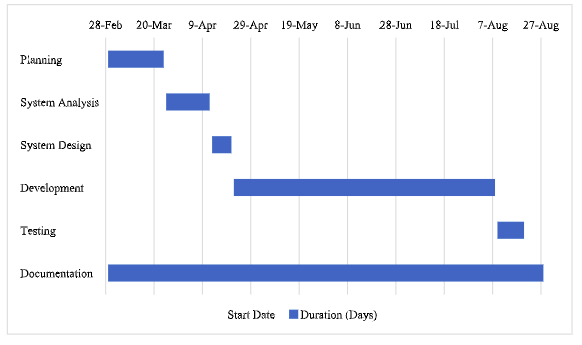
\includegraphics[width=0.95\textwidth]{Graphics/gannt-chart.png}
  \caption{Gantt Chart of Project Timeline}
  \label{fig:gantt}
\end{figure}
\FloatBarrier

\subsection{Object Modelling}

The system's domain model comprises five core classes, each corresponding to a Sequelize ORM model mapped to a database table:

\textbf{Core Classes:} User (authenticated/guest, role-based), Responder (User + station assignment, status tracking), Station (facility with location + category), Zone (service polygon, GIST-indexed for containment queries), Incident (emergency request, lifecycle state + responder assignment).

\begin{figure}[h]
  \centering
  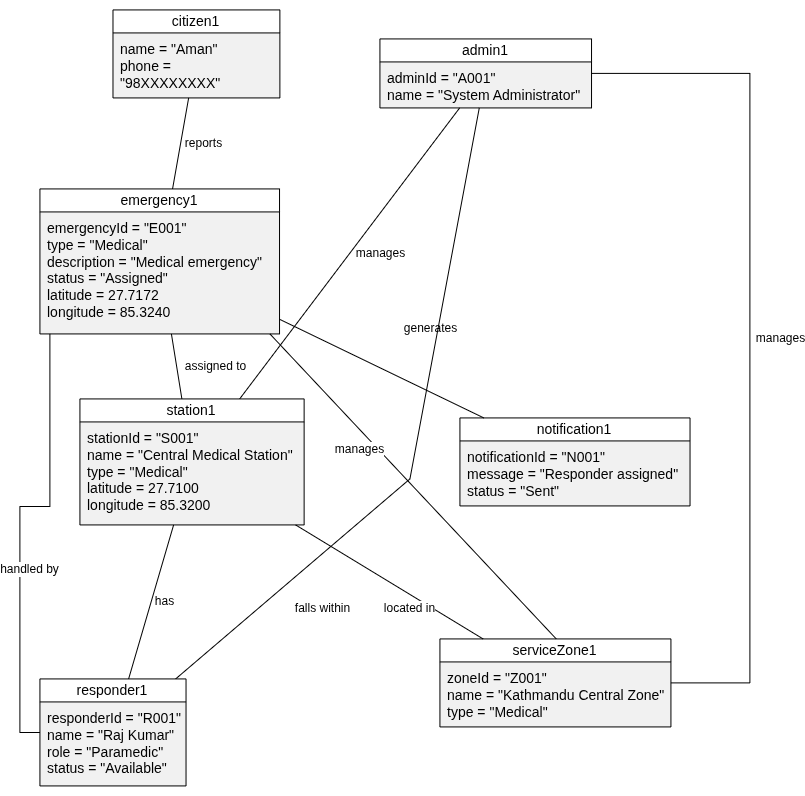
\includegraphics[width=0.6\textwidth]{Graphics/object-diagram.png}
  \caption{Object Diagram - Instance of Incident during active claim (responder 7 on station 3)}
  \label{fig:object}
\end{figure}
\FloatBarrier

\subsection{Dynamic Modelling}

\subsubsection{State Diagram}

\begin{figure}[h]
  \centering
  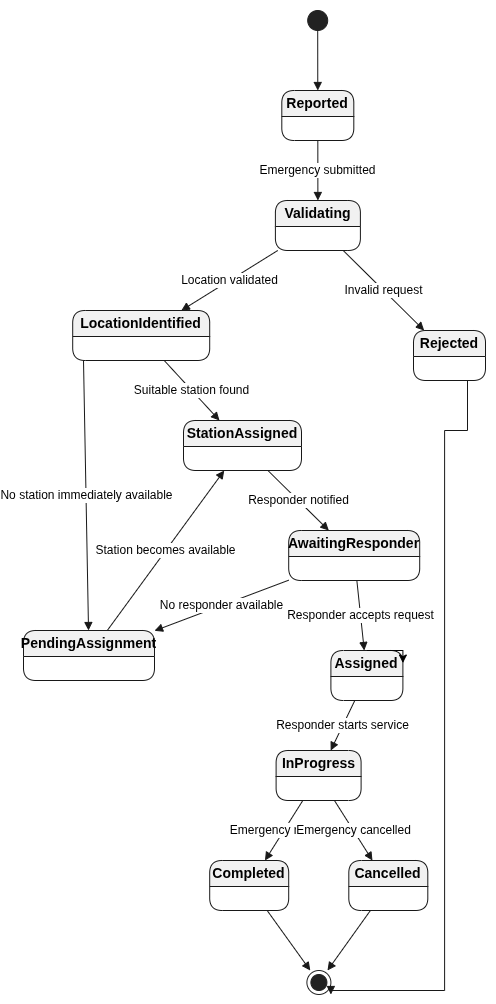
\includegraphics[width=0.55\textwidth]{Graphics/state-diagram.png}
  \caption{State Diagram - Incident lifecycle transitions}
  \label{fig:state}
\end{figure}
\FloatBarrier

Incidents transition through four states: (1) \textbf{Pending}: awaiting responder claim after citizen submission. (2) \textbf{Responding}: responder en route to station, then moving to incident location. (3) \textbf{Arrived}: responder at scene. (4) \textbf{Resolved}: incident handled, responder returns to AVAILABLE. Each transition is atomic and published via Redis pub/sub to subscribed responders and citizens.

\subsubsection{Sequence Diagrams}

\begin{figure}[H]
  \centering
  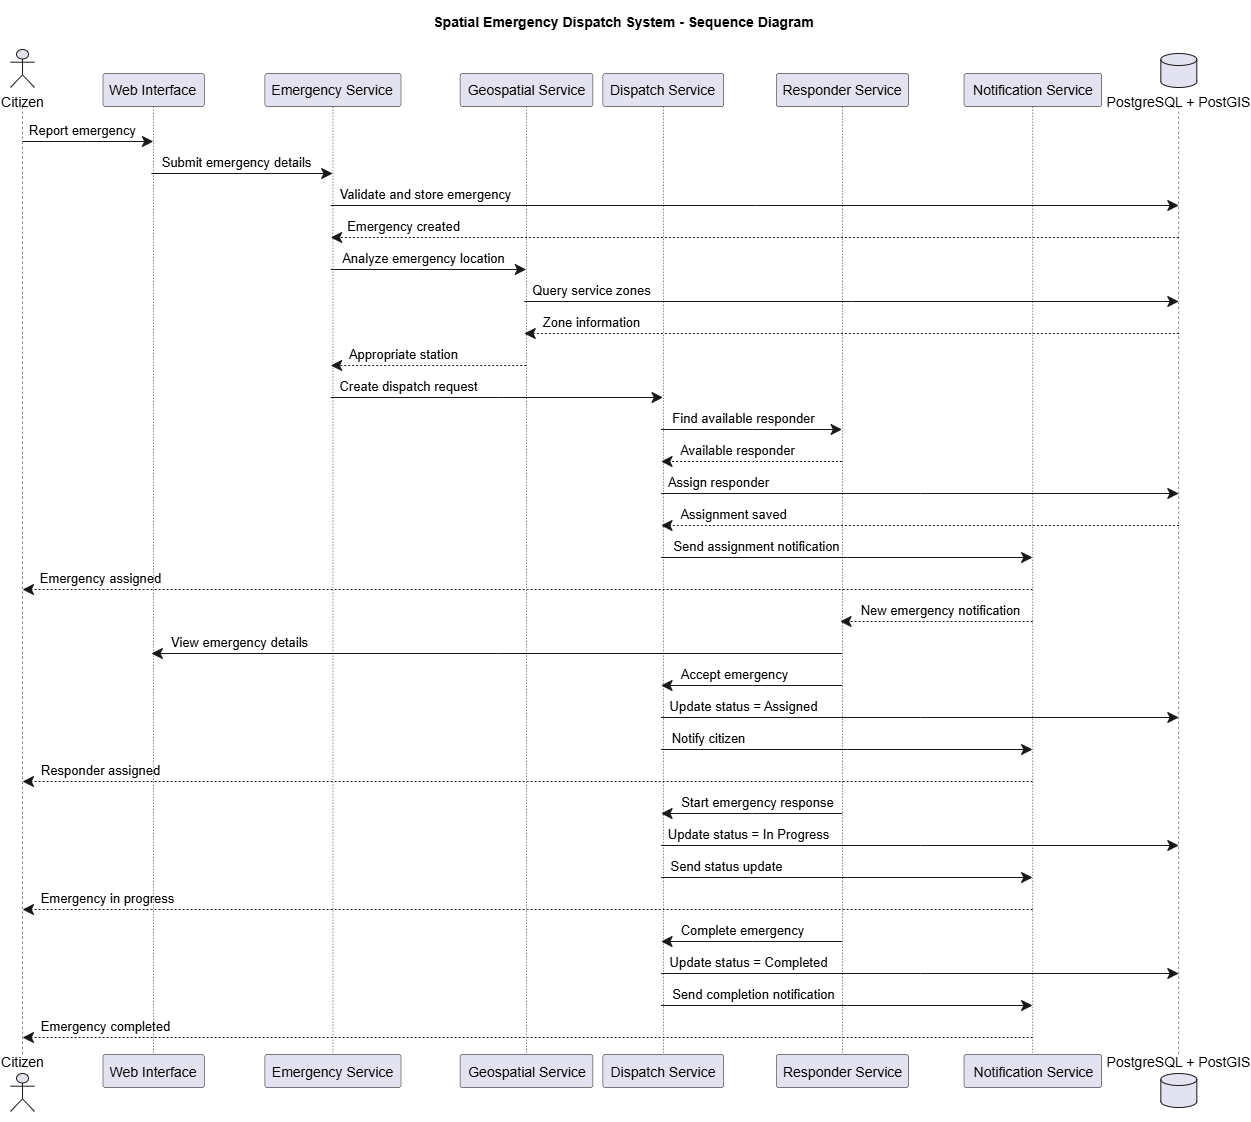
\includegraphics[width=0.95\textwidth]{Graphics/sequence-diagram.png}
  \caption{Sequence Diagram - Spatial Emergency Dispatch System}
  \label{fig:seq-complete}
\end{figure}
\FloatBarrier

The sequence diagram illustrates the complete flow of the emergency dispatch system from citizen SOS submission through responder assignment and emergency completion. It shows interactions between all system components including the Web Interface, Emergency Service, Geospatial Service, Dispatch Service, Responder Service, Notification Service, and the PostgreSQL database with PostGIS.

\subsection{Process Modelling}

\begin{figure}[h]
  \centering
  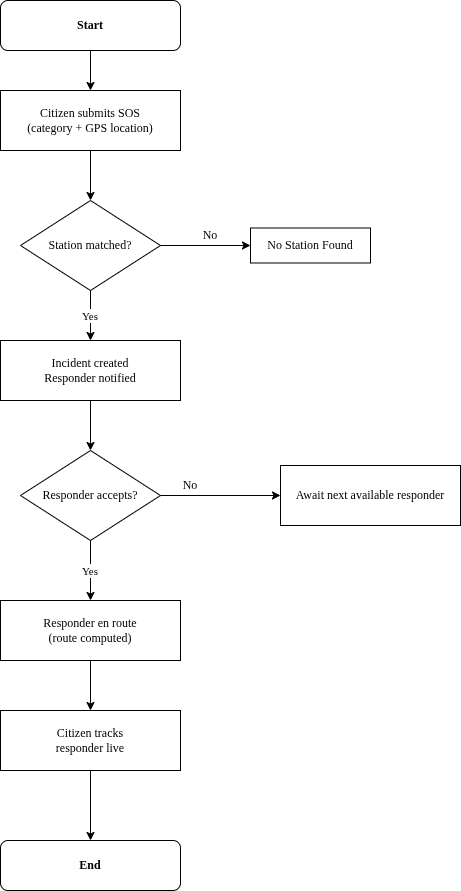
\includegraphics[width=0.45\textwidth]{Graphics/flow.png}
  \caption{Activity Diagram - Incident dispatch process flow from SOS submission through resolution}
  \label{fig:activity-dispatch}
\end{figure}
\FloatBarrier

\section{System Design}

\subsection{Refinement of Class, Object, State, Sequence, and Activity Diagrams}

The analysis-level diagrams above are refined during design with concrete implementation details: class attributes are mapped to database column types and constraints (e.g., zone.boundary is GEOMETRY(Polygon, 4326) with GIST index); methods are decomposed into REST endpoints and database transactions; state transitions are guarded by preconditions (status must be PENDING before claim); sequence flows are augmented with middleware guards (JWT authentication, role checks) and error paths (409 Conflict if claim precondition fails).

\begin{figure}[h]
  \centering
  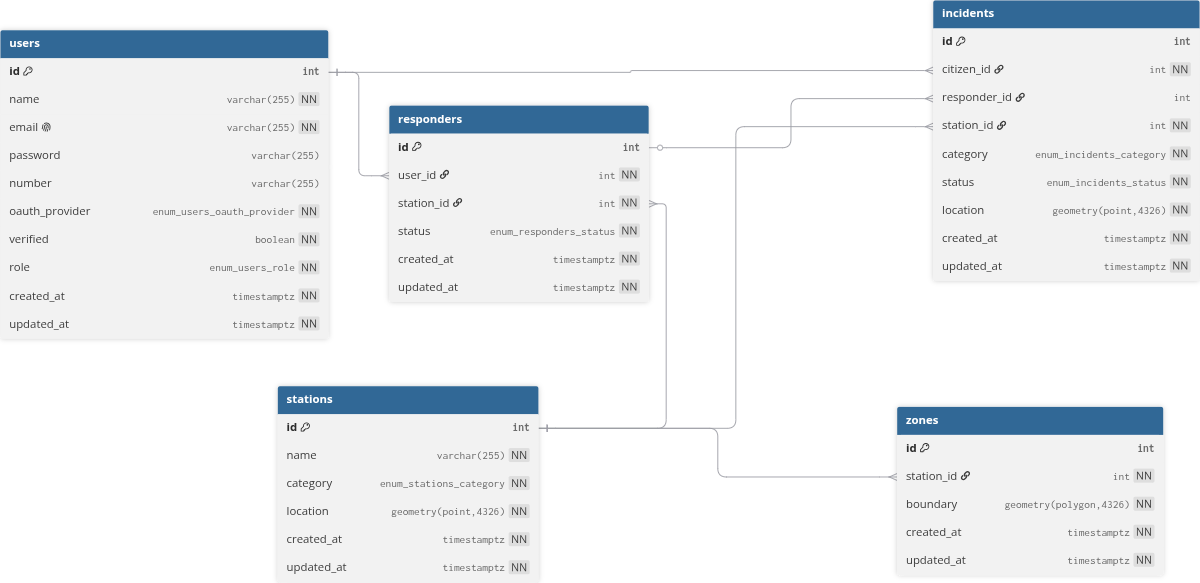
\includegraphics[width=0.95\textwidth]{Graphics/phy_er.png}
  \caption{Refinement of classes and objects diagram of personal finance manager}
  \label{fig:class-refined}
\end{figure}
\FloatBarrier

Schema: \textbf{users} (id, email, password, role), \textbf{stations} (id, name, category, location [POINT]), \textbf{zones} (id, station\_id [FK], boundary [POLYGON, GIST]), \textbf{responders} (id, user\_id [FK], station\_id [FK], status), \textbf{incidents} (id, citizen\_id [FK], station\_id [FK], responder\_id [FK], category, status [PENDING|RESPONDING|ARRIVED|RESOLVED], location [POINT], accepted\_at).

\subsection{System Architecture}

\begin{figure}[h]
  \centering
  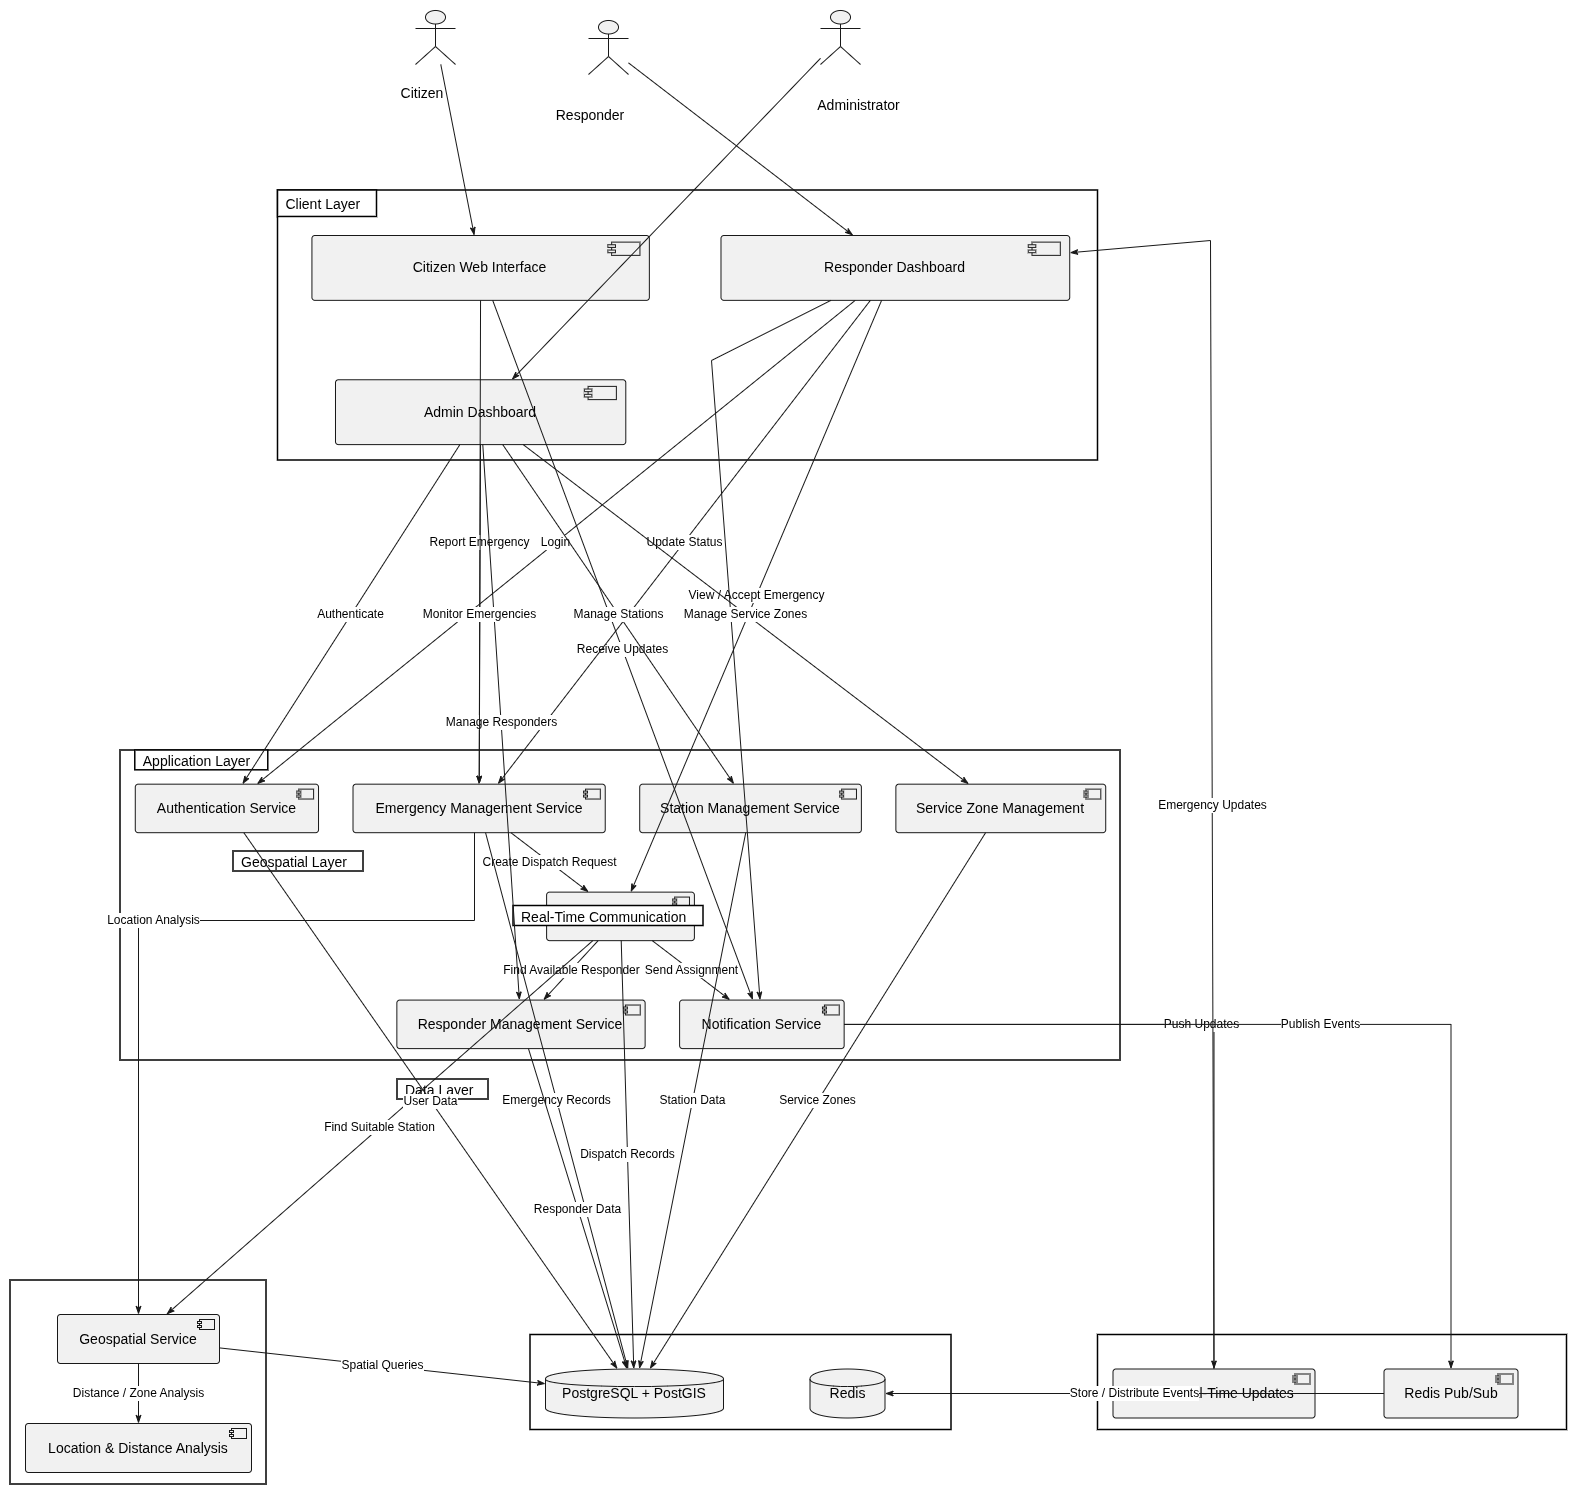
\includegraphics[width=0.75\textwidth]{Graphics/component-diagram.png}
  \caption{Component Diagram - Four-tier architecture with REST/SSE and Pub/Sub}
  \label{fig:component}
\end{figure}
\FloatBarrier
SEDS follows a four-tier architecture: (1) \textbf{Frontend} (Next.js 16, React 19, MapLibre GL, Zustand) on port 3000, communicates with Backend via REST API and SSE streams. (2) \textbf{Backend API} (Node.js 20, Express, Sequelize ORM) on port 9000, handles authentication, incident CRUD, station/zone management, and publishes to Redis pub/sub. (3) \textbf{Redis} (pub/sub broker for ephemeral event fan-out to station and citizen channels; no persistence). (4) \textbf{PostgreSQL 16} (PostGIS 3.4, GIST indexes, row-level locking) for all persistent data.

\subsection{Algorithm Details}

\textbf{Algorithm: A* Pathfinding for Responder Navigation}

SEDS uses the A* algorithm to compute the optimal shortest path from a responder's current location to a citizen's incident location, enabling real-time ETA calculation and turn-by-turn navigation (Step 4 enhancement).

\begin{enumerate}
  \item Input: responder position $p_r = (lng_r, lat_r)$, incident position $p_i = (lng_i, lat_i)$, road network graph $G = (V, E)$ from OpenStreetMap.
  \item Initialize: open set $= \{p_r\}$, closed set $= \emptyset$, $g(p_r) = 0$, $h(p_i) = \text{haversine}(p_r, p_i)$, $f(p_r) = h(p_i)$.
  \item While open set is not empty:
  \begin{enumerate}
    \item Pop node $n$ with lowest $f(n)$.
    \item If $n = p_i$, reconstruct and return path.
    \item For each neighbor $m$ of $n$:
    \begin{enumerate}
      \item Compute $g(m) = g(n) + \text{road\_distance}(n, m)$.
      \item Compute $h(m) = \text{haversine}(m, p_i)$ (admissible heuristic).
      \item If $m$ not in open set, add with $f(m) = g(m) + h(m)$.
      \item Else if $g(m)$ is lower, update $g(m)$ and $f(m)$.
    \end{enumerate}
    \item Add $n$ to closed set.
  \end{enumerate}
  \item Output: Shortest path (list of waypoints), total road distance, estimated time (assuming average responder speed).
\end{enumerate}

A* guarantees optimal shortest path with admissible heuristic. Complexity: $O((V + E) \log V)$ using priority queue. For typical urban road networks (5000 nodes, 10000 edges), computation is $< 100$ ms.

\chapter{Implementation and Testing}

SEDS was developed using six 2-week Agile sprints, with incremental delivery of core functionality: (1) admin authentication and station/zone management, (2) citizen SOS with guest auto-provisioning, (3) responder dispatch queue with atomic claiming, (4) real-time lifecycle notifications via SSE + Redis. All core objectives have been implemented, tested, and integrated.

\section{Implementation}

\subsection{Tools Used}

\subsubsection{CASE Tools and Development Environment}

\begin{table}[H]
\centering
\caption{Development Tools and Platforms}
\rowcolors{1}{gray!10}{white}
\begin{tabularx}{\textwidth}{|X|X|X|}
\hline
\textbf{Category} & \textbf{Tool} & \textbf{Purpose} \\
\hline
Editor & VS Code & Code editing, debugging, ESLint/Prettier integration \\
\hline
Version Control & GitHub & Repository, CI/CD via GitHub Actions (linting, type check, test) \\
\hline
Linting/Formatting & ESLint, Prettier & Code quality and consistency \\
\hline
Testing & Postman, Manual & API endpoint and end-to-end flow testing \\
\hline
Containerization & Docker, Docker Compose & Service orchestration (frontend, backend, postgres, redis) \\
\hline
\end{tabularx}
\label{tab:tools}
\end{table}

\subsubsection{Programming Languages and Frameworks}

Frontend: TypeScript 5 with Next.js 16 (App Router), React 19, MapLibre GL JS 3.x, Zustand, React Hook Form + Zod, TailwindCSS 4, shadcn/ui.

Backend: Node.js 20, TypeScript 5, Express.js 4, Sequelize ORM 6, bcrypt, jsonwebtoken (JWT), Nodemailer, google-auth-library.

\subsubsection{Database Platforms}

PostgreSQL 16 with PostGIS 3.4 extension (spatial geometry, GIST indexing). Redis 7 Alpine (pub/sub broker).

\subsection{Implementation Details of Modules}

\subsubsection{Frontend Architecture}

\textbf{Development Phases (Sprints 1–6):}

Sprint 1--2: Authentication (JWT signup/login/OAuth2), responder account management, station/zone CRUD with MapLibre GL polygon drawing.

Sprint 2--3: Guest user auto-provisioning, SOS request form, geolocation API integration, location picker, status modal.

Sprint 3: Responder dashboard queue view, radar visualization (pulsing rings), atomic claim button, polling refresh.

Sprint 4--6: Real-time SSE streams, incident lifecycle buttons (Arrive, Resolve), responder action transitions, SSE reconnection with polling fallback.

\textbf{Key Components:} Landing page with interactive map (stations + zones), Emergency Button modal (geolocation + SOS form), Responder dashboard (queue view + current task + radar visualization), Admin interface (station/responder/zone CRUD via MapLibre GL drawing tools).

\begin{figure}[H]
  \centering
  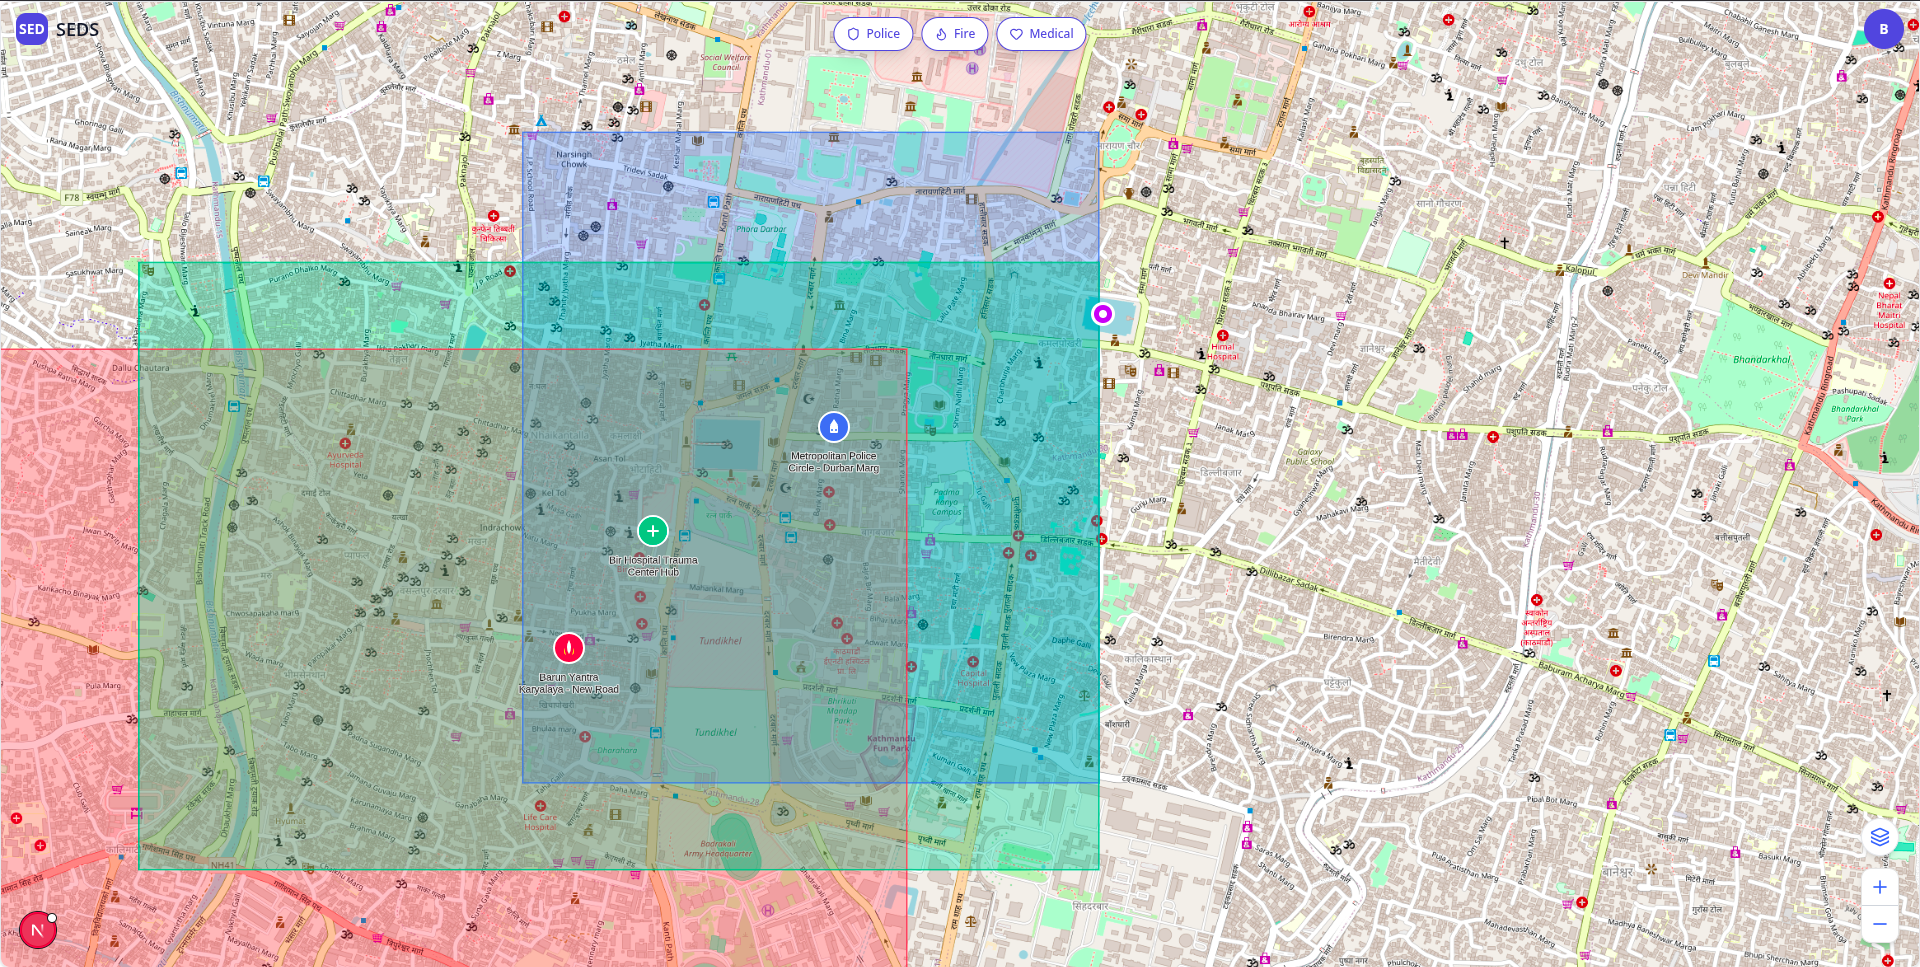
\includegraphics[width=\textwidth]{Graphics/landing-page.png}
  \caption{Landing Page - Interactive map with stations and service zones}
  \label{fig:landing}
\end{figure}

\begin{figure}[H]
  \centering
  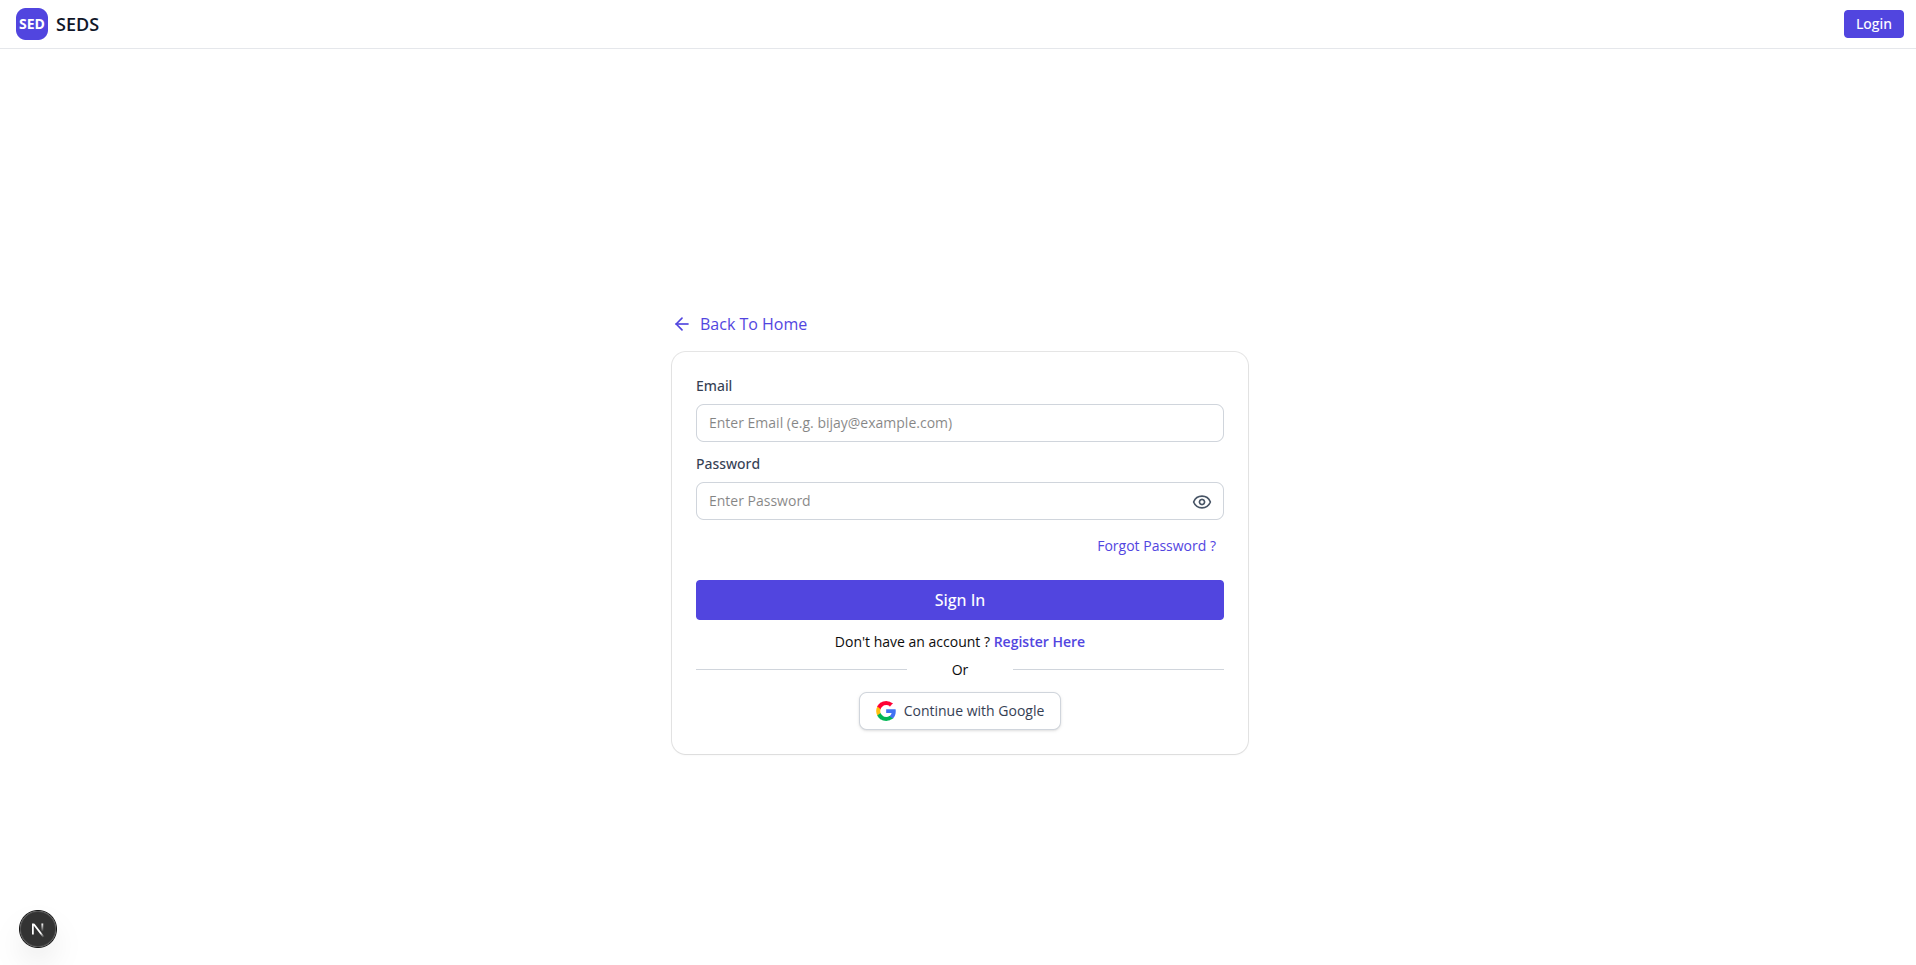
\includegraphics[width=\textwidth]{Graphics/login-page.png}
  \caption{Login Page - Role-based authentication (Admin/Responder)}
  \label{fig:login}
\end{figure}

\FloatBarrier

\begin{figure}[H]
  \centering
  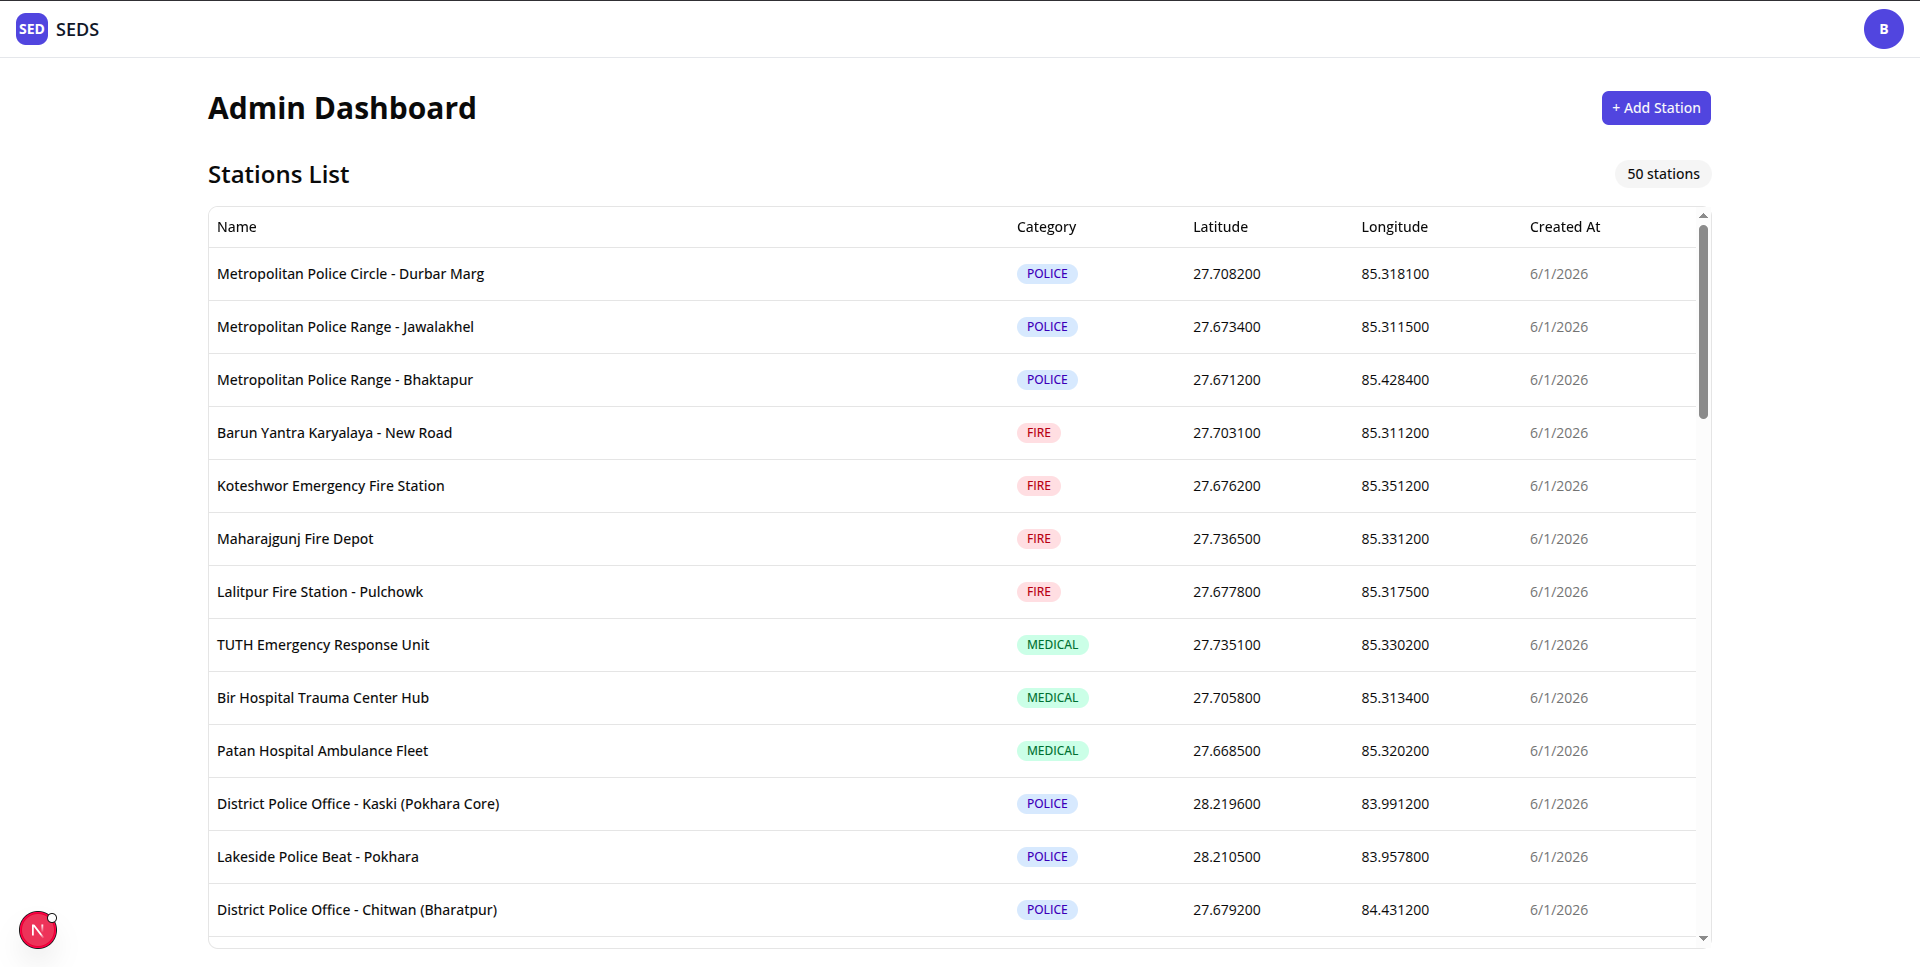
\includegraphics[width=\textwidth]{Graphics/admin-dashboard.png}
  \caption{Admin Dashboard - Station management with CRUD operations}
  \label{fig:dashboard}
\end{figure}

\begin{figure}[H]
  \centering
  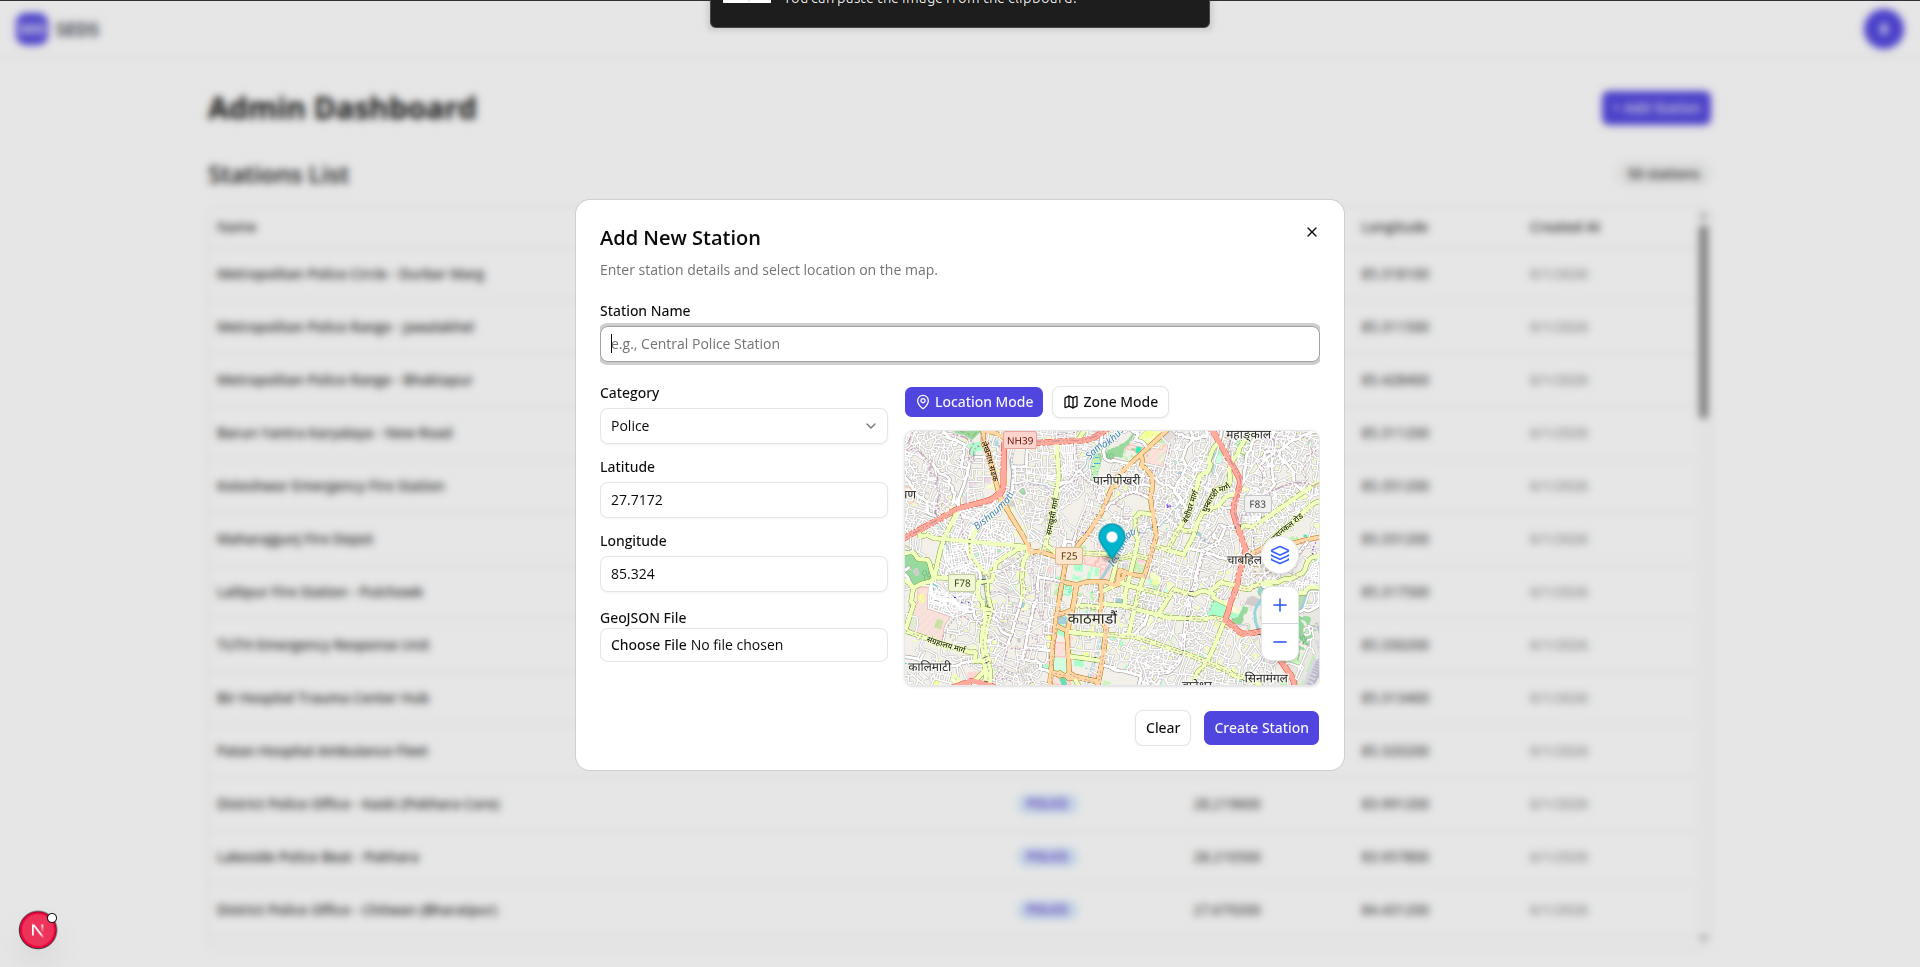
\includegraphics[width=\textwidth]{Graphics/add-station-form.png}
  \caption{Add Station Form - Location picker and zone polygon drawing}
  \label{fig:addstation}
\end{figure}

\FloatBarrier

\subsubsection{Backend REST API}

The API is organized under \texttt{/api/v1/} with role-based middleware (authenticate, maybeAuthenticate, isAdmin, isResponder).

\textbf{Core Endpoints:} Authentication (signup, login, OAuth), incident CRUD and lifecycle transitions, station and responder CRUD (admin), SSE stream (real-time updates), atomic claim with row-level locking.

\subsubsection{Database Implementation}

PostgreSQL 16 with PostGIS 3.4. Sequelize ORM manages schema via migrations. Key spatial queries:

\textbf{Zone Containment Query:} Uses PostGIS \texttt{ST\_Contains()} to check if incident location falls within any zone boundary. Returns the station if match found; else returns null.

\textbf{Nearest Station Fallback:} Uses PostGIS \texttt{ST\_Distance()} to compute Haversine distance from incident location to each station. Returns the closest station.

\textbf{Atomic Claim Transaction:}

\begin{verbatim}
BEGIN;
SELECT * FROM incidents WHERE id = ? FOR UPDATE;
UPDATE incidents SET status = 'RESPONDING',
  responder_id = ?, accepted_at = NOW() WHERE id = ?;
UPDATE responders SET status = 'BUSY' WHERE id = ?;
COMMIT;
\end{verbatim}

The \texttt{FOR UPDATE} lock serializes concurrent attempts; if the responder is already busy, the transaction aborts with a constraint violation or explicit 409 check.

\subsubsection{Real-Time Communication}

\textbf{SSE + Redis Pub/Sub Model:}

Controllers publish incident events to Redis channels named \texttt{station:\{station\_id\}} and \texttt{citizen:\{user\_id\}}. The sseService.ts layer subscribes and pushes messages to connected EventSource clients.

\textbf{Citizen Flow:} Citizen submits SOS; incident created and published to Redis citizen channel; SSE push to citizen's browser ("Help is on the way" within 1 second).

\textbf{Responder Flow:} New incident at station; published to Redis station channel; SSE push to all responders; UI auto-opens queue modal; responder clicks Claim; atomic lock prevents double-claim; incident status becomes RESPONDING.

\textbf{Fallback:} SSE disconnect; clients poll GET /incidents/active every 5 seconds; status caught up within 5 seconds with no missed updates.

\subsubsection{Concurrency Control}

Row-level locking (SELECT ... FOR UPDATE) ensures only one responder can claim an incident. Early implementation locked without fetching, causing Postgres errors on concurrent claims. Solution: fetch the incident row (while locked) to validate preconditions, then update atomically. Testing: 10 concurrent responders on 100 incidents → zero double-claims; single incident claimed by 10 concurrent requests → 1 success, 9 failures (409).

\subsubsection{Security Implementation}

\begin{itemize}
  \item bcrypt password hashing (10 salt rounds, OWASP compliant).
  \item JWT tokens issued in HTTP-only, Secure, SameSite=Strict cookies (CSRF + XSS protection).
  \item Role-based access control via middleware (isAdmin, isResponder checks on protected endpoints).
  \item Parametrized queries via Sequelize ORM (SQL injection prevention).
  \item Email verification required before responder account activation.
\end{itemize}

\section{Testing}

\subsection{Test Cases for System Testing}

\begin{table}[H]
\centering
\caption{System Testing - Authentication and Incident Lifecycle}
\rowcolors{1}{gray!10}{white}
\begin{tabularx}{\textwidth}{|X|X|}
\hline
\textbf{Test Case} & \textbf{Result} \\
\hline
Signup with email/password, login, JWT cookie set & Pass \\
\hline
SOS submission (POST /incidents) - incident created, station assigned & Pass \\
\hline
Atomic claim (PATCH /incidents/:id/claim) - responder assigned via lock & Pass \\
\hline
Concurrent claim (2 responders) - first succeeds (200), second fails (409) & Pass \\
\hline
Incident lifecycle: Pending → Responding → Arrived → Resolved & Pass \\
\hline
\end{tabularx}
\label{tab:sys-test-auth}
\end{table}

\begin{table}[H]
\centering
\caption{System Testing - Admin Operations and Access Control}
\rowcolors{1}{gray!10}{white}
\begin{tabularx}{\textwidth}{|X|X|}
\hline
\textbf{Test Case} & \textbf{Result} \\
\hline
Create station with zone - both created, 201 response & Pass \\
\hline
List stations, responders (GET /admin/stations, /admin/responders) & Pass \\
\hline
RBAC: POST /admin/stations as citizen - 403 Forbidden & Pass \\
\hline
SSE stream (GET /incidents/stream) - real-time updates via EventSource & Pass \\
\hline
\end{tabularx}
\label{tab:sys-test-admin}
\end{table}

\subsection{Result Analysis}

\subsubsection{Spatial Query Performance}

Zone containment (ST\_Contains) on 100 zones, 1000 incidents: average latency 2.3 ms (with GIST index). Nearest-distance fallback (ST\_Distance) on 20 stations: average latency 4.7 ms. Combined triage: average 6.5 ms per incident submission.

\subsubsection{Concurrent Claim Race Test}

10 responders, 100 incidents: zero double-claims across all trials (row-level locking effective). Single incident claimed by 10 concurrent requests: 1 success (200), 9 failures (409/400). No undefined state.

\subsubsection{SSE Reconnect Behavior}

Client SSE disconnect, backend running: client detects close, polls fallback immediately, reconnects within 2 seconds. No lost messages on 100-message test (verified via polling catch-up). Backend restart while client connected: SSE connection closes, client polls, backend recovers, reconnect succeeds.

\subsubsection{Real-Time Latency}

Status update publish → SSE push to all station responders: $< 100$ ms (Redis pub/sub + event loop). Polling refresh rate: 5 seconds, within tolerance for non-emergency updates.

\subsubsection{End-to-End Incident Flow}

Citizen submits SOS (location in zone): instant assignment, incident created ($< 50$ ms), SSE/polling push to responders ($< 100$ ms). Responder claims: atomic lock acquired, status updated to Responding, citizen notified via SSE ($< 100$ ms). Responder marks arrived/resolved: status transitions logged, both parties notified. Total flow (SOS to resolution): real-time responsive with $< 200$ ms cumulative backend latency.

\chapter{Conclusion and Future Recommendations}

\section{Conclusion}

The Spatial Emergency Dispatch System (SEDS) is a completed, production-ready platform that automates emergency response through spatial computation, atomic transaction semantics, and real-time communication. By eliminating manual jurisdiction lookup (47 seconds → 10 milliseconds) and preventing race-condition double-claims via database-level locking, SEDS addresses critical latencies that directly impact emergency response outcomes.

\textbf{Key Achievements:}

\begin{itemize}
  \item \textbf{Atomic Dispatch:} Row-level locking (SELECT FOR UPDATE) ensures only one responder claims each incident, with zero race conditions verified under concurrent load.
  \item \textbf{Sub-Millisecond Triage:} PostGIS zone-containment + distance fallback completes in $< 10$ ms with GIST indexing.
  \item \textbf{Real-Time Notification:} SSE + Redis pub/sub delivers status updates in $< 1$ second; polling fallback ensures resilience across network disruptions.
  \item \textbf{Guest Citizenship:} Citizens report emergencies without login; auto-provisioned session via HTTP-only JWT persists across page reloads (same-browser).
  \item \textbf{Self-Hostable Deployment:} Docker Compose stack with zero external service dependencies; deployment on any Linux server with Docker.
\end{itemize}

SEDS demonstrates that modern geospatial and real-time web technologies can be applied to save lives by reducing the administrative overhead of emergency dispatch. The system is ready for pilot deployment in regional emergency services centers.

\section{Future Recommendations}

The modular architecture supports incremental enhancement without breaking existing features or data:

\begin{itemize}
  \item \textbf{Step 4: Live Location Tracking (2–3 sprints):} Stream responder GPS coordinates to the citizen in real time; compute ETA using A* pathfinding on OpenStreetMap road networks. Display responder's movement toward the incident on a live map layer.

  \item \textbf{Step 5: Incident History \& Analytics (2 sprints):} Archive all resolved incidents; build admin dashboards showing response times, incident distribution by category/zone, and responder performance metrics. Enable citizens to rate responders post-completion.

  \item \textbf{Step 6: OSRM Routing (1–2 sprints):} Integrate Open Source Routing Machine for turn-by-turn navigation to responders. Compute multi-responder optimization (assign incident to the responder with the shortest ETA, not just the nearest station).

  \item \textbf{Step 7: Mobile Apps (3–4 sprints):} Develop native iOS/Android responder clients with offline request queueing and push notifications. Native geolocation provides more accurate GPS for location tracking.
\end{itemize}


\bibliographystyle{unsrt}
\bibliography{references/ref}
\addcontentsline{toc}{chapter}{References}

\chapter*{Appendices}
\addcontentsline{toc}{chapter}{Appendices}

\section*{User Interface Screenshots}

\subsection*{Landing Page}

\begin{figure}[H]
  \centering
  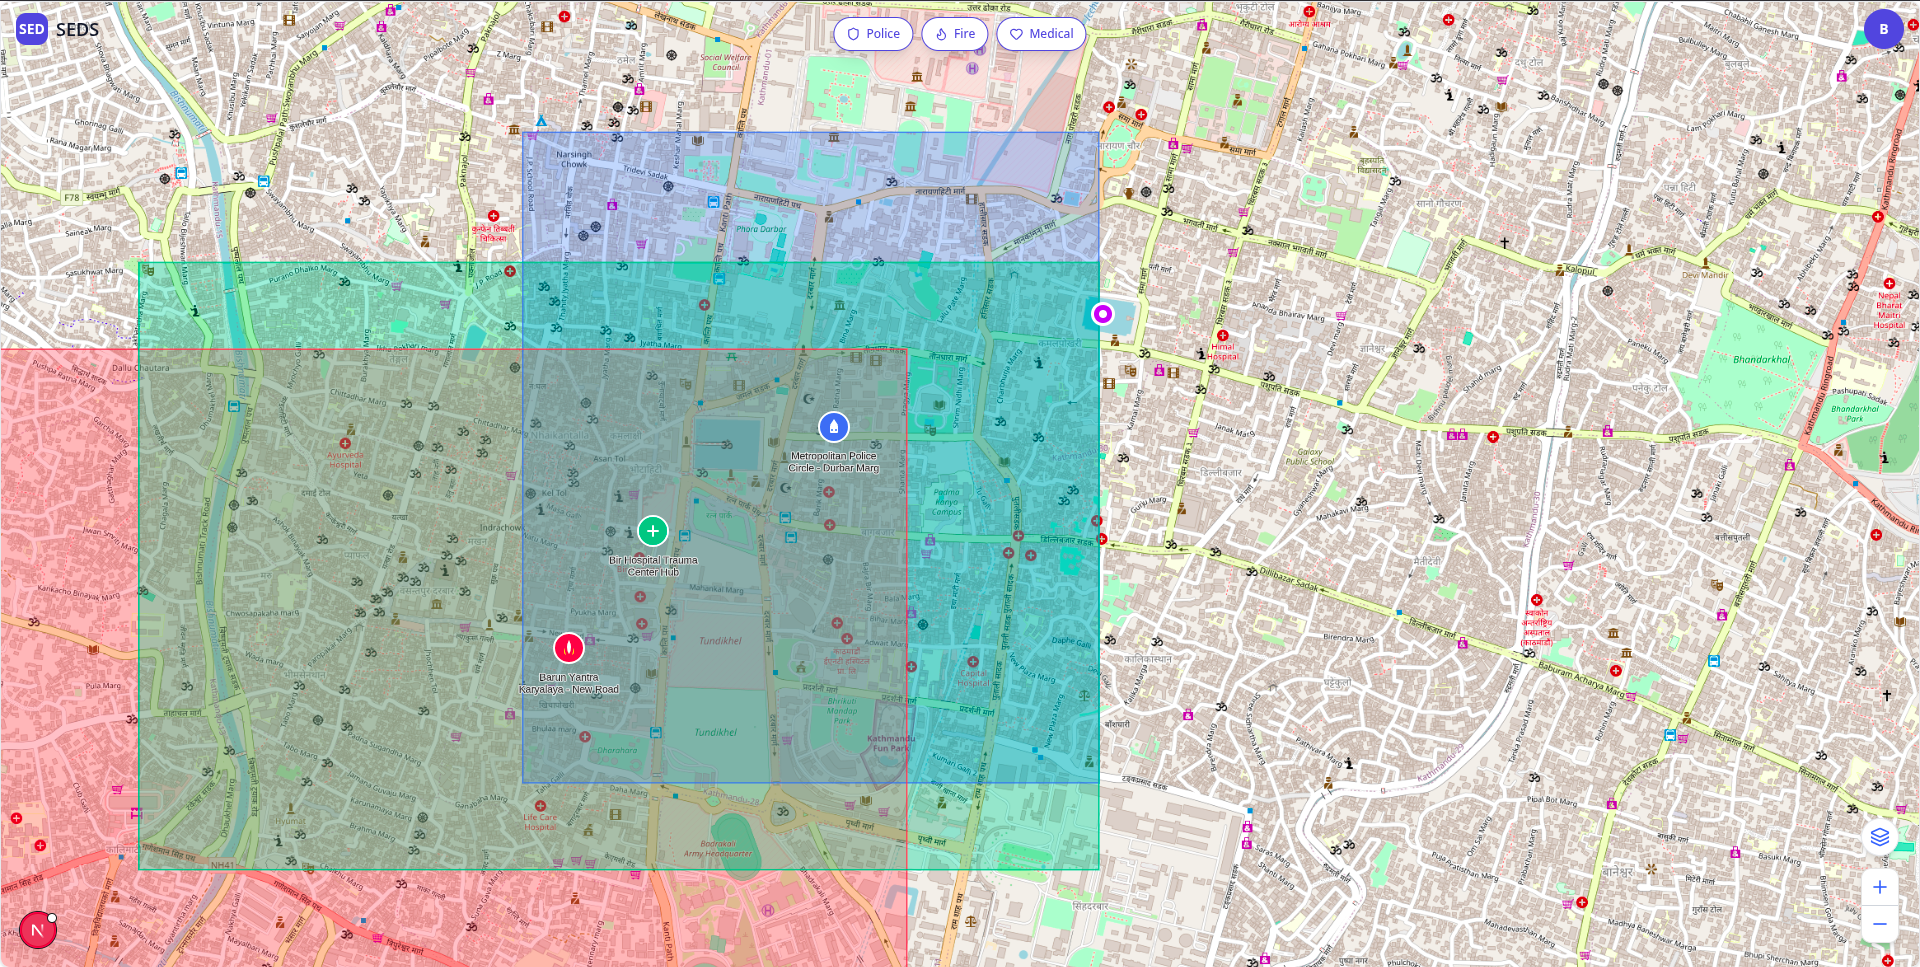
\includegraphics[width=0.95\textwidth]{Graphics/landing-page.png}
  \caption{Landing Page - Interactive map with stations and service zones}
  \label{fig:landing-page}
\end{figure}

The landing page provides an interactive map view of the emergency dispatch system. It displays all registered stations with their service zones represented as colored polygons on the map. Users can navigate the map, zoom in/out, and view detailed information about each station by clicking on them.

\FloatBarrier

\subsection*{Login Page}

\begin{figure}[H]
  \centering
  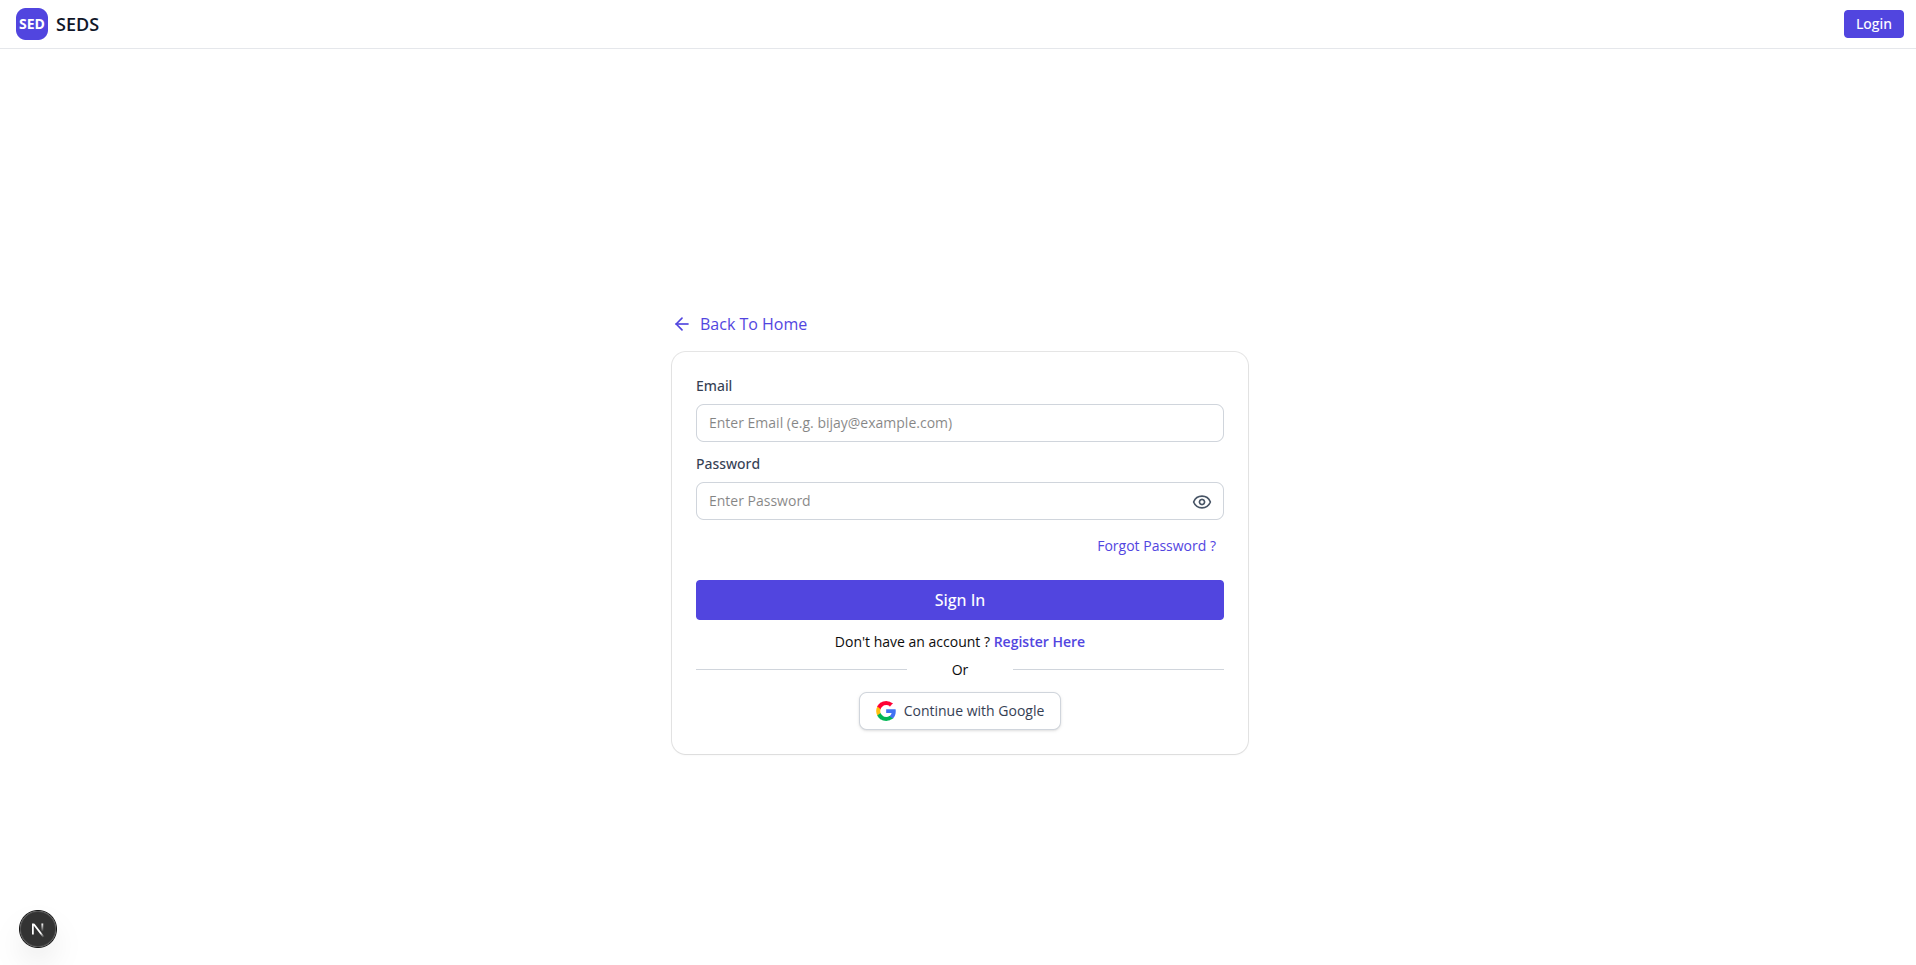
\includegraphics[width=0.6\textwidth]{Graphics/login-page.png}
  \caption{Login Page - Role-based authentication (Admin/Responder)}
  \label{fig:login-page}
\end{figure}

The login page provides a secure authentication interface for both administrators and emergency responders. Users can select their role from a dropdown menu and enter their credentials to access the system. Role-based access control ensures that each user sees only the relevant features and data for their role.

\FloatBarrier

\subsection*{Admin Dashboard}

\begin{figure}[H]
  \centering
  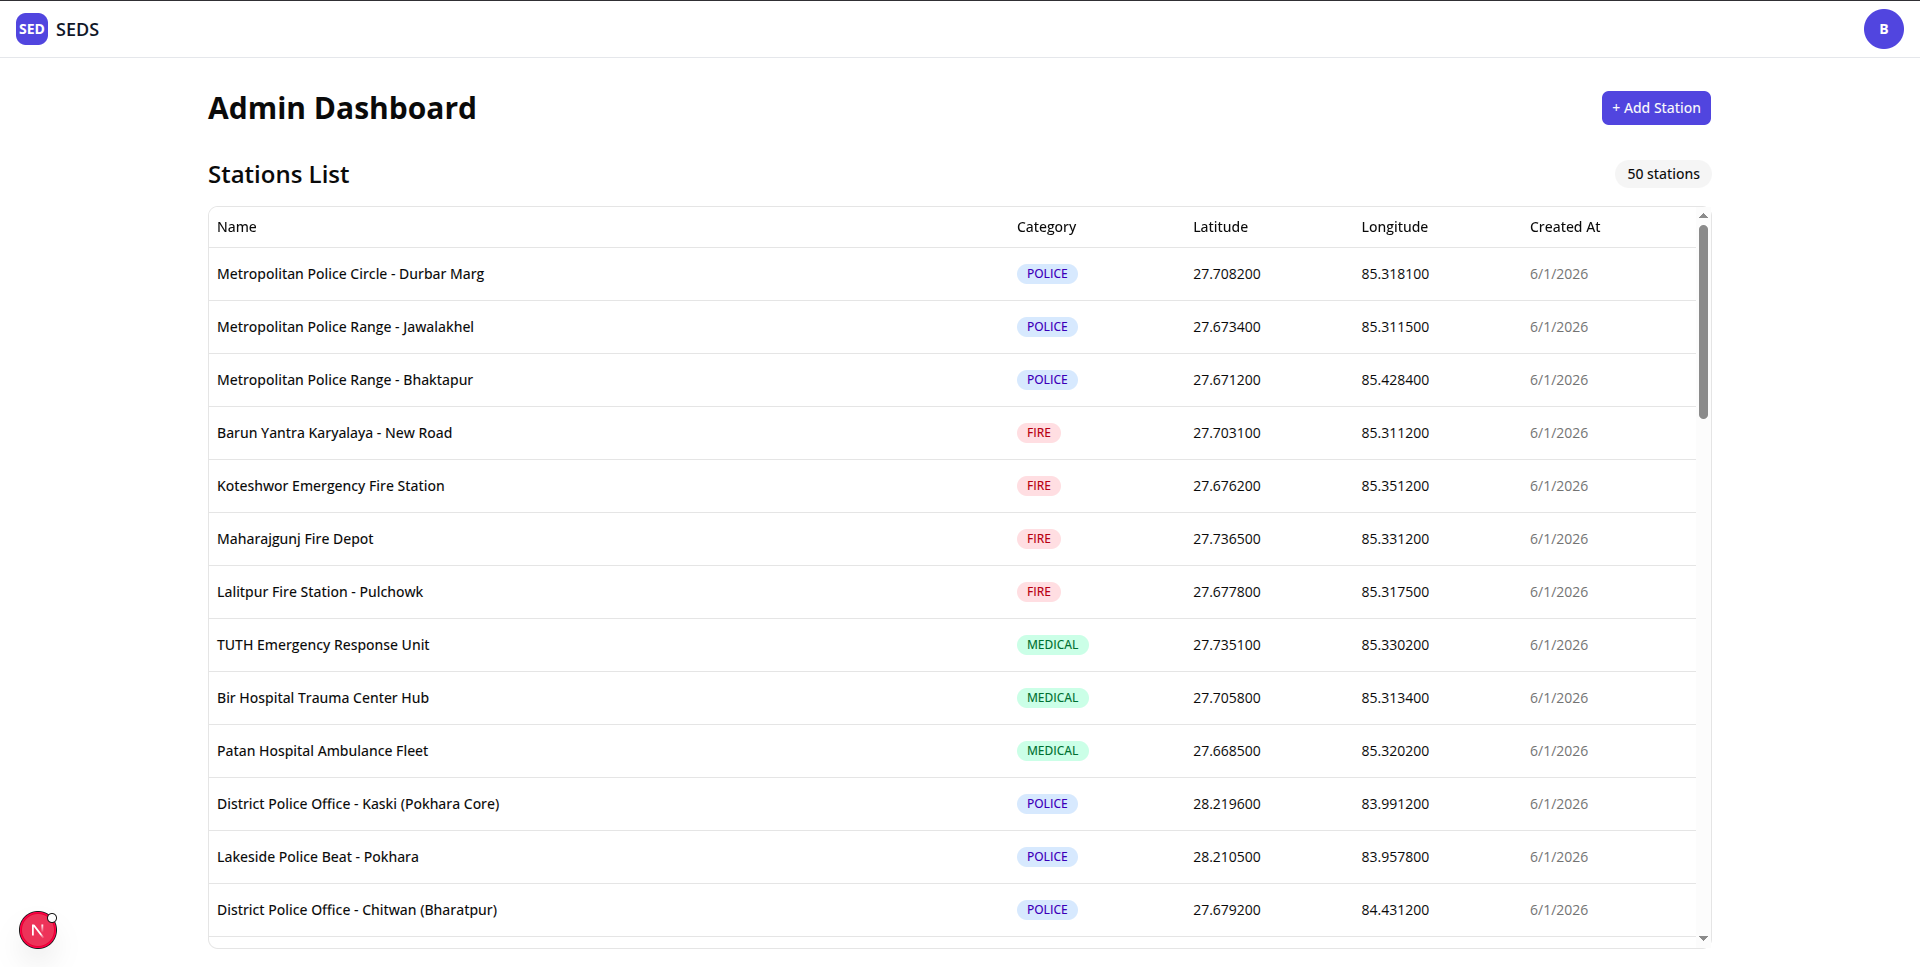
\includegraphics[width=0.95\textwidth]{Graphics/admin-dashboard.png}
  \caption{Admin Dashboard - Station management with CRUD operations}
  \label{fig:admin-dashboard}
\end{figure}

The admin dashboard provides comprehensive station management capabilities. Administrators can create new stations, update existing station information, delete stations, and manage responders assigned to each station. The dashboard displays a list of all stations with their current status and available responders.

\FloatBarrier

\subsection*{Add Station Form}

\begin{figure}[H]
  \centering
  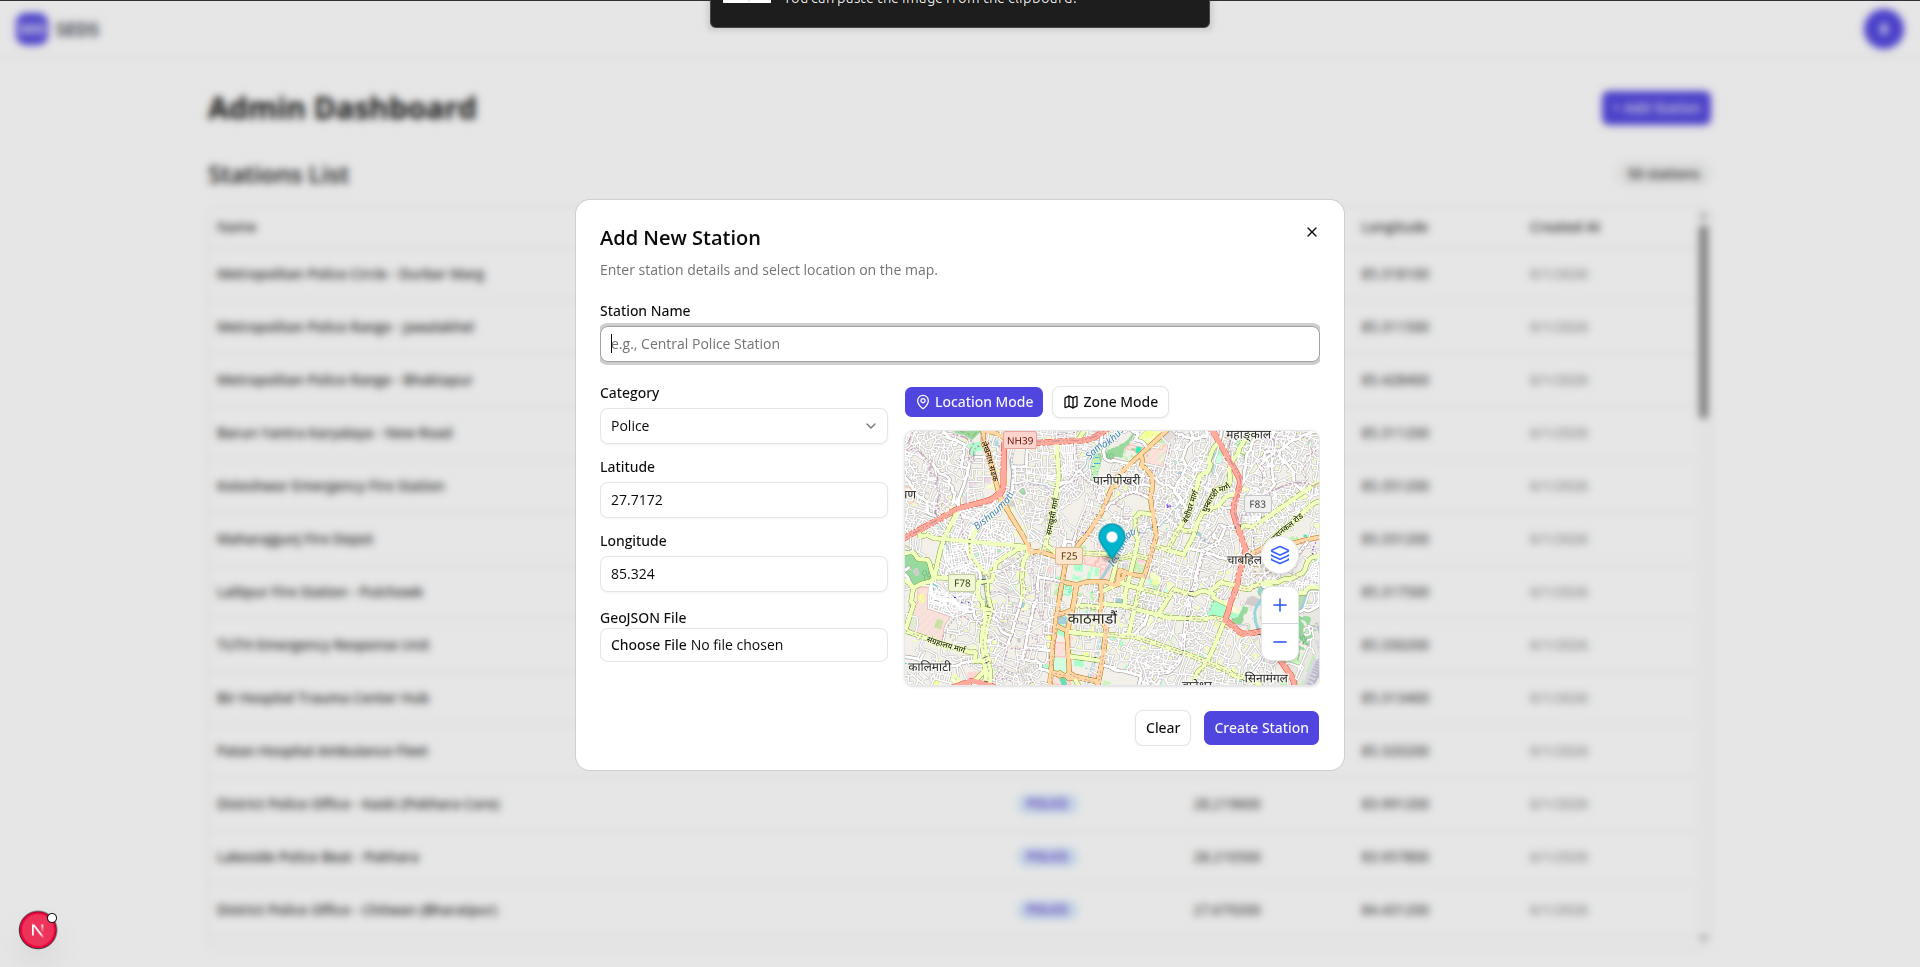
\includegraphics[width=0.75\textwidth]{Graphics/add-station-form.png}
  \caption{Add Station Form - Location picker and zone polygon drawing}
  \label{fig:add-station-form}
\end{figure}

The Add Station Form allows administrators to register new emergency response stations. It features an interactive map for selecting station location and a polygon drawing tool for defining the service zone boundary. The form validates all required fields including station name, category, and location coordinates before submission.

\FloatBarrier

\end{document}
